\documentclass[12pt]{article}
\usepackage{fontspec}   %加這個就可以設定字體
\usepackage{amsmath}
\usepackage{amsfonts}
\usepackage{xeCJK}
\usepackage{amsbsy}
\usepackage{caption}
\usepackage{multirow}
\usepackage{subfigure}
\usepackage{titlesec}
\usepackage{titletoc}
\usepackage{CJKnumb}
\usepackage{color} 
\usepackage{pdfpages} % include outside .pdf
\usepackage{wallpaper}
\usepackage[hidelinks]{hyperref}
\newcommand{\sectionbreak}{\clearpage}
\setCJKmainfont{標楷體}
\renewcommand{\tablename}{表}%表標題中文化
\renewcommand{\figurename}{圖}%圖標題中文化
%\renewcommand{\bibname}{\B 參考文獻}%參考文獻中文化
\renewcommand {\thetable} {\thesubsection{}.\arabic{table}}
\renewcommand {\thefigure} {\thesubsection{}.\arabic{figure}}
\renewcommand {\theequation} {\thesubsection{}.\arabic{equation}}
\newcommand{\topcaption}{%
\setlength{\abovecaptionskip}{0pt}%
\setlength{\belowcaptionskip}{2pt}%
\caption}%圖標題用caption至於下方, 表標題則用topcaption
\renewcommand{\baselinestretch}{1.5}
\titleformat{\section}[hang]{\centering\Large\bf}{第\,\CJKnumber{\thesection}\,章}{0.1cm}{}
\titlecontents{section}[0em]{}{\makebox[4.1em][l]{第\xCJKnumber{\thecontentslabel}章}}{}{\titlerule*[0.7pc]{.}\contentspage}
\XeTeXlinebreaklocale "zh" 
\XeTeXlinebreakskip = 0pt plus 1pt
\newfontfamily\timesbd{Times New Roman Bold}
\usepackage{graphicx}
\usepackage{natbib}%使用參考文獻
\usepackage{booktabs}
\author{林澤慶}
\bibliographystyle{plain}%使用TER格式列出參考文獻
\renewcommand{\refname}{\ctxfbb 參考文獻}
\renewcommand\contentsname{目~錄}
\renewcommand\listfigurename{圖次}
\renewcommand\listtablename{表次}
\renewcommand\abstractname{摘~要}
\renewcommand\figurename{圖~}
\renewcommand\tablename{表~}
\renewcommand\bibname{參~考~文~獻}

\begin{document}
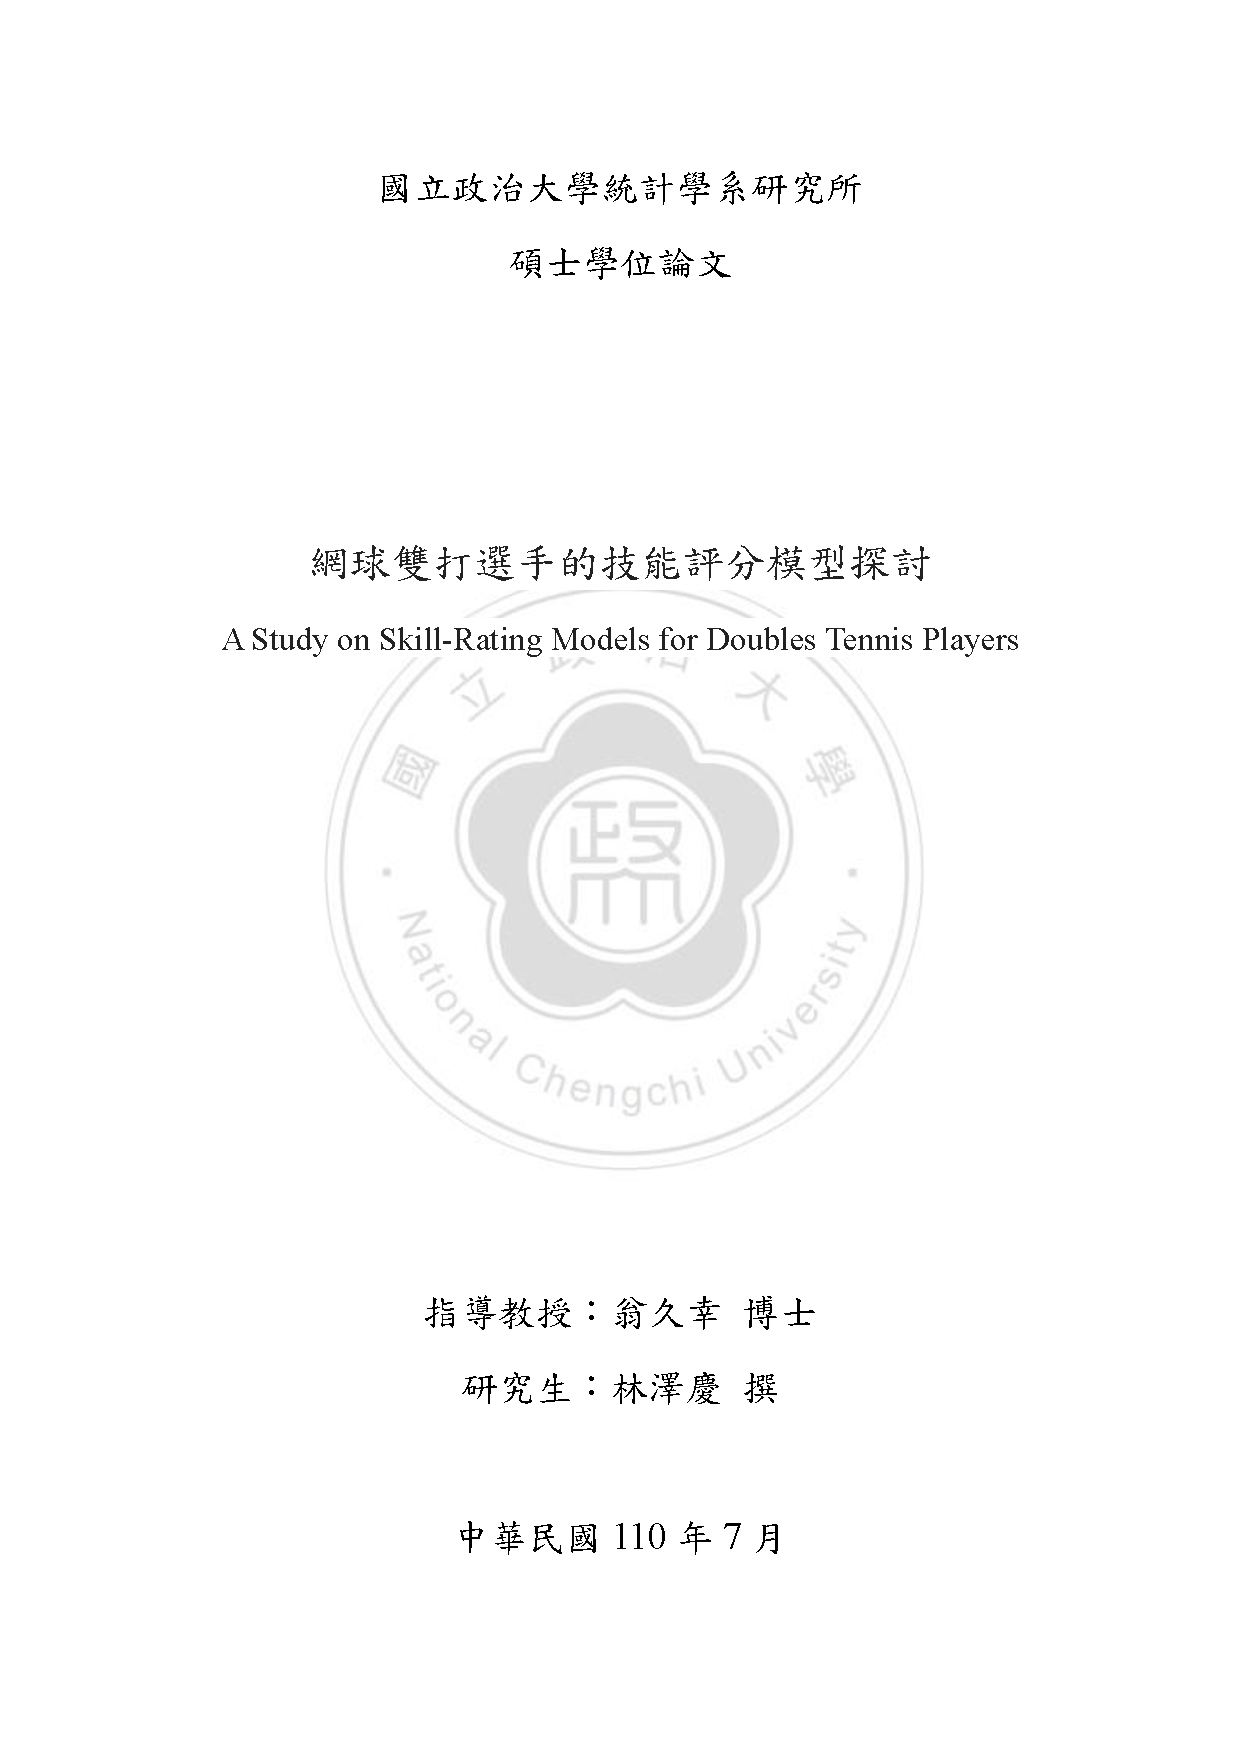
\includepdf[pages=1-3]{cover.pdf}
% 政大論文浮水印
% 政大論文浮水印
% \CenterWallPaper{0.174}{pdfs/watermark.pdf}
% \setlength{\wpXoffset}{6.1725cm}
% \setlength{\wpYoffset}{10.5225cm}

\CenterWallPaper{}{pdfs/watermark.pdf}
\setlength{\wpXoffset}{0pt}
\setlength{\wpYoffset}{0pt}
% Table of Content
\clearpage
\tableofcontents
% List of Figures
\clearpage
\listoffigures
% List of Tables
\clearpage
\listoftables
%\mainmatter
\section{緒論}
\subsection{研究動機}

網球一直被視為一種熱門的運動,從基層的學校網球社團、網球校隊、業餘的網球俱樂部,甚至到職業的網球比賽,皆有網球的活動。隨著網球運動的興起,越來越多的網球好手參加職業網球比賽,其中又以四大網球公開賽為主,分別是澳洲網球公開賽(Australian Open)、法國網球公開賽(French Open)、溫布敦網球公開賽(The Championships, Wimbledon)、美國網球公開賽(U.S. Open),此外,我國好手也曾屢次獲得亮眼的表現,例如:詹皓晴與詹詠然在泰國芭達雅公開賽(Thailand Open)拿下冠軍,盧彥勳曾在馬哈拉施特拉邦公開賽(Maharashtra Open)獲得雙打冠軍。
	
隨著越多的好手在球場上發揮精湛的技術,除了有線電視的直播與網路直播的興起,搭配運動彩券的帶動下,網球比賽的討論度也越來越高,一些網球愛好者除了討論球員發揮的技術以外,亦會討論球員之間的比賽結果,甚至會投入資金於運動彩券,並且支持他們喜愛的球員,倘若能建立一個預測模型,並能有效預測球員間的比賽結果,因此,人們可以透過投注運動彩券,將此模型預測球員間的比賽結果,並在運動彩券上獲利。

過去在討論預測職業網球比賽模型的文獻主要是以單打居多,例如:蕭立承\cite{hsiao2020}撰寫的職業網球單打評分模型的實證研究、Ingram	\cite{Ingram+2021}撰寫的How to extend Elo: a Bayesian perspective等文獻,這些文獻皆有建立評分模型,以衡量各選手所發揮的實力,並且預測網球選手之間的比
賽結果,然而討論職業網球雙打的評分模型的文獻偏少,因此本人想要研究職業網球雙打的評分模型。

\subsection{研究目的}
過去在常見評分模型有Bradley-Terry model\cite{10.2307/2334029}、Elo model\cite{elo1978rating}、Glicko model\cite{alma991021119382005721}等,這些模型皆可以評估參賽隊伍的實力。職業網球選手的實力發揮往往會受到比賽場地的因素而受到影響,本論文改良Bradley-Terry模型,並且讓模型能考慮到比賽場地的效應,讓模型能有效的運用在職業網球雙打比賽上。
\section{文獻回顧}
\subsection*{配對比較(Paired Comparison)}
配對比較(Paired comparison)方法為彼此互相比較,也就是將不同的配對進行比較,常用於運動競賽、遊戲比賽等。常用配對比較模型有Elo評分系統與Glicko評分系統,起初,Elo評分系統用在職業西洋棋比賽,其用來評估選手的實力,後來,Glicko評分系統亦運用在西洋棋比賽上,至今,運動賽事也常採用配對比較方法來評估參賽者的實力,本節會介紹Elo評分系統與Glicko評分系統。
\subsection{Elo}
Arpad Elo提出Elo \cite{elo1978rating} 評分系統(Elo rating system),其調整的方式為:
\[
new\  winner\  rating = old\   winner\  rating + k * (1-P(win))
\]
\[
new\  loser\  rating = old\   loser\  rating + k * (1-P(win))
\]
其中獲勝機率$P(win)$代表藉由邏輯函數(logistic function)估計運動員獲勝的機率,$k$代表可以控制的常數,一般而言,$k$會設定為32,每一位參賽者的評分起始值設定為1500,透過上述的方式調整每位參賽選手的評分。
\\
\\
根據Elo評分系統,第i位參賽者的勝率為(\ref{equ:1})式:
\begin{equation}
p(y = 1 | \hat{\theta}_i,\hat{\theta}_j) = \frac{1}{1+10^{-(\hat{\theta}_i-\hat{\theta}_j)/400}} 
\label{equ:1}
\end{equation}
參賽者的評分更新方式為(\ref{equ:w})式和(\ref{equ:l})式:
\begin{equation}
\hat{\theta}^{'}_w = \hat{\theta}_w + k \times (1 - p(y = 1|\hat{\theta}_w,\hat{\theta}_j))
\label{equ:w}
\end{equation}
\begin{equation}
\hat{\theta}^{'}_l = \hat{\theta}_l - k \times (1 - p(y = 1|\hat{\theta}_w,\hat{\theta}_j))
\label{equ:l}
\end{equation}
(\ref{equ:w})式和(\ref{equ:l})式中$\hat{\theta}_w$與$\hat{\theta}_l$分別代表更新前贏家的評分與輸家的評分,$\hat{\theta}^{'}_w$與$\hat{\theta}^{'}_l$分別代表更新後贏家的評分與輸家的評分,並顯示自贏家的評分會被向上調整$k \times (1-p(y = 1|\hat{\theta}_w,\hat{\theta}_j))$,輸家的評分會被向下調整$k \times (1-p(y = 1|\hat{\theta}_w,\hat{\theta}_j))$,更新後的贏家評分與輸家評分之合與更新前的贏家評分與輸家評分之合相同,故贏家評分與輸家評分之合維持一定於Elo評分系統。
\subsection{Glicko}
由 Glickman 提出Glicko評分系統 \cite{alma991021119382005721},其模型是一種於配對比較方法,此模型主要貢獻評分可靠性(Ratings Reliability)。Glicko評分系統會根據每個時間點賦予每位參賽者實力參數$\theta$,其會隨著時間變化而受到波動。
假設開始的參賽者實力參數服從常態分配,表示如下:
\begin{equation}
\theta_i|\sigma^2_0 \sim N(1500,\sigma^2_0)
\end{equation}
在時間$t_0$下,參賽者實力參數分布如下:
\begin{equation}
\theta^{(t_0)}|\mu,\sigma^2 \sim N(\mu,\sigma^2)
\label{equ:glickot0}
\end{equation}
時間$t_0$下,經過時間$t$個單位,第$i$位參賽者實力參數分布如下:
\begin{equation}
\theta^{(t_0+t)}_i|\theta^{(t_0)}_i,\nu^2,t \sim N(\mu,\nu^2t)
\label{equ:glickot0+t}
\end{equation}
根據(\ref{equ:glickot0})與(\ref{equ:glickot0+t})的結果,參賽者實力可更新如下:
\begin{equation}
\theta^{(t_0+t)}|\mu,\sigma^2,\nu^2,t \sim N(\mu,\sigma^2 + \nu^2 t)
\label{equ:rate}
\end{equation}
上述(\ref{equ:rate})式說明參賽者實力的變異性會隨著時間增加而增加,接下來透過更新的演算法,找出常態分配的$\mu$、$\sigma^2$的更新方法,其更新的方式如下:
\begin{equation}
\mu' = \mu + \Sigma_{j=1}^m \Sigma_{k=1}^{n_j}{g(\sigma^2_j)[s_{jk}-E(s|\mu,\mu_j,\sigma^2_j)]}
\label{equ:update}
\end{equation}
\begin{equation}
\sigma'^2 = (\dfrac{1}{\sigma^2} + \dfrac{1}{\delta^2})^{-1}
\end{equation}
其中
\[
b = log(10)/400
\]
\[
g(\sigma^2) = \dfrac{1}{\sqrt{1+3b^2\sigma^2/\pi^2}}
\]
\begin{equation}
E(s|\mu,\mu_j,\sigma^2_j) = \dfrac{1}{1+10^{-g(\sigma^2_j)(\mu-\mu_j)/400}}
\label{equ:expect}
\end{equation}
\[
\delta^2 = [b^2 \Sigma_{j=1}^m{n_jg(\sigma^2_j)^2E(s|\mu,\mu_j,\sigma^2_j)[1-E(s|\mu,\mu_j,\sigma^2_j)]}]^{-1}
\]
上述(\ref{equ:expect})式代表參賽者碰到第$j$位參賽者預期會獲勝的機率,(\ref{equ:update})式為事後評分的更新方式,其更新的方法與Elo評分系統更新的方式相似,會透過比賽結果與期望會獲勝的機率來調整參賽者的實力,若預期獲勝的機率與實際比賽結果差異過大,則參賽者實力會有較大幅調整。

\section{研究方法}

\subsection{Bradley-Terry Model}
Bradley \& Terry提出Bradley-Terry Model\cite{10.2307/2334029},此為一種可評估排名的機率模型,其可以用來估計成隊的比賽,透過參賽者的實力計算獲勝機率,其機率模型如下:
\begin{equation}
P(X_i > X_q) = \dfrac{\pi_i}{\pi_i + \pi_q}
\label{equ:bt}
\end{equation}
其中$X_i>X_q$代表第$i$隊隊伍擊敗第$q$隊隊伍,$P(X_i>X_q)$代表第$i$隊隊伍擊敗第$q$隊隊伍的機率,$\pi_i$代表第$i$隊隊伍的實力,$\pi_q$代表第$q$隊隊伍的實力,此外,仍須滿足每一隊隊伍的評分$\pi$皆須大於等於0且$\Sigma{\pi_i}=1$。

假設每一場比賽結果是互相獨立的,第$i$隊隊伍與第$q$隊隊伍在第$k$次對戰中,其發生對戰結果機率如下:
\begin{equation}
(\dfrac{\pi_i}{\pi_i+\pi_q})^{r_{iqk}}(\dfrac{\pi_q}{\pi_i + \pi_q})^{1-r_{iqk}}
\label{equ:b-t}
\end{equation}
在(\ref{equ:b-t})式中,$r_{iqk}$代表第$i$隊隊伍與第$q$隊隊伍在第$k$次對戰中的比賽結果,當比賽結果是第$i$隊隊伍擊敗第$q$隊隊伍時,則$r_{iqk}=1$,反之,當第$q$隊隊伍擊敗第$i$隊隊伍時,則$r_{iqk}=0$。

經過了n場比賽後,根據每一場比賽的結果資訊,我們可以獲得其概似函數,其概式函數呈現如下:
\begin{equation}
L(\mathbf{\pi}) = \prod_{i<j}\prod_k(\dfrac{\pi_i}{\pi_i+\pi_q})^{r_{iqk}}(\dfrac{\pi_q}{\pi_i + \pi_q})^{1-r_{iqk}}
\label{equ:likeli}
\end{equation}

我們可以透過($\ref{equ:likeli}$)式估計每一隊隊伍的實力$\pi$。

Bradley-Terry 模型(\ref{equ:bt})可以用若干不同方式推得,其中一種是令$X_i$服從Gumbel分配,其累積密度函數為
\[
P(X_i \leq x) = exp(-exp(-(x-\theta_i))), \theta_i = log \pi_i
\]
則$X_i-X_q$服從邏輯斯分配,其累積密度函數為
\[
P(X_i-X_q \leq x) = \dfrac{e^{\theta_q}}{e^{\theta_i-x}+e^{\theta_q}}
\]
當$x = 0$,則
\[
P(X_i > X_q) = 1-P(X_i \leq X_q) = \dfrac{e^{\theta_i}}{e^{\theta_i}+e^{\theta_q}} = \dfrac{{\pi_i}}{{\pi_i}+{\pi_q}}
\],即為(\ref{equ:bt})式。
\subsection{GenElo Surface Model}

職業網球選手會因為場地的不同材質,而影響到參賽者的實力發揮,網球場地的材質基本上可以分成3類,分別是紅土(Clay)、草地(Grass)與硬地(Hard)。紅土球場的特性在於球速較為緩慢,有比較多的時間追球,對於防禦型底線型球員有較好的發揮空間,草地球場的特性在於球落地時有較小的摩擦力,且不時會有不規則的彈跳,對於發球上網型球員有較佳的發揮空間,硬地球場的特性在於球的彈跳速度快,因此讓對手有較少的反應時間,對於侵略型底線型球員較具有優勢。

GenElo Surface Model由Ingram\cite{Ingram+2021}將Elo評分模型進行擴增,此模型是將Elo評分模型考慮了比賽場地的因素,讓模型除了參考雙方選手的實力以外,亦會將比賽的結果與場地資訊當作參考依據。

為了讓模型能配適場地的變數,首先先考慮一場中的輸家與贏家的實力,參賽者的先驗實力服從常態分配,其分配如下:
\begin{equation}
\boldsymbol{\theta_w \sim N(\mu_w,\Sigma); \theta_l \sim N(\mu_l, \Sigma)}
\label{dis:w_l}
\end{equation}
在(\ref{dis:w_l})式中,$\boldsymbol{\theta_w}$與$\boldsymbol{\theta_l}$皆為長度為$n$的向量,分別代表贏家與輸家在$n$種不同場地上的實力,$\mu_w$與$\mu_l$皆為長度為$n$的向量,$\Sigma$為$n * n$的矩陣,其代表在不同場地之間,參賽者評分的共變異數矩陣,且假設無論是贏家或輸家皆有共同的共變異數矩陣$\Sigma$,比方,以網球比賽而言,場地可能是紅土、草皮、硬地等,分別給予編號$1,2,3$號。

在假設贏家與輸家的實力彼此獨立的情況下,$\boldsymbol{\theta_w}$與$\boldsymbol{\theta_l}$的聯合分配如下:
\begin{equation}
\boldsymbol{\theta = \begin{bmatrix}
\theta_w \\ \theta_l \end{bmatrix} \sim N\left(\begin{bmatrix}
\mu_w \\ \mu_l
\end{bmatrix},\begin{bmatrix}
\Sigma & 0 \\ 0 & \Sigma
\end{bmatrix}
\right) = N(\mu_{\theta},\Sigma_{\theta})}
\end{equation}
我們介紹$\boldsymbol{a}$,其定義為:
\begin{equation}
\boldsymbol{a} = \begin{bmatrix}
\boldsymbol{a_w} \\ -\boldsymbol{a_l}
\end{bmatrix}
\label{equ:mat}
\end{equation}
在(\ref{equ:mat})式中,$\boldsymbol{a_w} = \boldsymbol{a_l}$,且皆為長度為$n$的dummy vector,在該比賽的場地指派為1,其餘則指派為0,比方,若該場地為第1種場地,則$\boldsymbol{a_w} = \boldsymbol{a_l} = (1,\underbrace{0,...,0}_{n-1 個})$。

根據貝氏定理(Bayes' rule),取對數的後驗機率正比如下:
\begin{equation}
t(\boldsymbol{\theta}) \propto - \dfrac{1}{2}\boldsymbol{(\theta-\mu_{\theta})^T\Sigma^{-1}_{\theta}(\theta - \mu_{\theta})} + log\gamma(b\boldsymbol{a^T\theta})
\label{postior}
\end{equation}
其中
\[
\gamma(x) =  logit^{-1}(x)
\]
\[
b = log(10)/400
\]
將(\ref{postior})式利用牛頓法(Newton's method)更新$\mu_{\theta}$,其更新的方法如下:
\begin{equation}
\boldsymbol{\mu'_{\theta}} = \boldsymbol{\mu_{\theta} - \textit{H}^{-1}(\mu_{\theta})j(\mu_{\theta})}
\label{update}
\end{equation}
在(\ref{update})式中$\textit{H}$和$j$分別代表$t(\boldsymbol{\theta})$的Hessian matrix與Jacobian,其中$\boldsymbol{\textit{H}(\mu_{\theta})}$與$\boldsymbol{j(\mu_{\theta})}$可以表示如下:
\begin{equation}
\boldsymbol{j(\mu_{\theta})} = (1-\gamma(b \boldsymbol{a^T \mu_{\theta}}))b \boldsymbol{a}
\label{jacob}
\end{equation}
\begin{equation}
\textit{H}(\boldsymbol{\mu_{\theta}}) = -\boldsymbol{\Sigma^{-1}_{\theta}} - \gamma(b \boldsymbol{a^T \mu_{\theta}})(1-\gamma(b \boldsymbol{a^T \mu_{\theta}}))b^2 \boldsymbol{aa^T}
\label{hessian}
\end{equation}
我們可以透過(\ref{update})、(\ref{jacob})與(\ref{hessian})式的更新方式,參賽選手的實力依照比賽結果進行調整。
\subsection{多組別多組員之比賽}
Weng \& Lin提出Bradley-Terry Model with full-pair 與partial pair\cite{JMLR:v12:weng11a}評分模型,該模型可以適用於$k \geq 2$組隊伍且每隊隊伍有多位選手的比賽。當$k = 2$且每隊有2人的情況,就是常見的雙打比賽。當$k > 2$,比方$k = 4$,代表有4組隊伍A,B,C,D。若一場比賽之結果,A,B,C,D依序為第1,第2,第3,第4,此結果可以用A贏B,B贏C,C贏D這3個兩兩比賽的結果代表;也可以用A贏B,B贏C,C贏D,A贏C,A贏D,B贏D這6個兩兩比賽的結果代表之。前者以$(k-1)$個兩兩比賽結果代表一場$k$隊比賽結果,稱之為partial-pair;後者以$C^k_2$個兩兩比賽結果代表一場$k$隊比賽結果,稱之為full-pair。不管是partial-pair或full-pair,在網球比賽$(k = 2)$得$k-1 = C^k_2 =1$,結果相同。每經過一場比賽後,可以將組內參賽選手的實力進行調整,令$X_i$代表第$i$隊的實際表現。比方在球場上的實際表現會因為天候、場地、球員的身體狀況而有所差別,所以可將$X_i$視為隨機變數。此模型是將Bradley-Terry Model進行擴充,讓模型能多考慮到變異數的部分,此模型為:
\begin{equation}
P(X_i > X_q) = \dfrac{e^{\theta_i/c_{iq}}}{e^{\theta_i/c_{iq}} +e^{\theta_q/c_{iq}}}
\end{equation}
其中
\[
c^2_{iq} = \beta^2_i + \beta^2_q\ 
\]
其中$\theta_i$代表第$i$隊的實力,$\beta_i$代表第i隊隊伍實際表現的不確定性,$c^2_{iq}$代表第i隊隊伍與第q隊隊伍之不確定性的加總。


假設第$i$隊的實力$\theta_i$亦為一隨機變數,且在比賽前其事前分配(prior distribution)為$N(\mu_i,\sigma^2_i)$。當比賽結束後,可以透過貝式方法估計第$i$隊實力的事後期望值與變異數,亦即更新隊伍實力的平均數與變異數。此模型假設各隊之$\mu_i$,$\sigma^2_i$分別為其隊員之事前平均數,事前變異數之加總,且假設$\beta^2_i = \sigma^2_i + \beta^2$,其中$\beta^2$是事先給定之正數。當$k =2$,亦即每場比賽僅有2組,其更新的演算法如下:
\\
步驟1:給定每一場比賽的結果s與每一隊隊伍中隊員的$\mu_{ij},\sigma^2_{ij}(i=1,2,j=1,2)$與$\beta^2,\kappa > 0$,並決定$\gamma_q$
\\
步驟2:針對一場比賽中每一隊計算$\mu_i,\sigma^2_i(i=1,2)$
\[
\mu_i = \Sigma^{2}_{j=1}\mu_{ij}, \sigma^2_i = \Sigma^{2}_{j=1}\sigma^2_{ij}
\]
步驟3:針對一場比賽中每一隊團隊評分與個人實力進行調整
\\
步驟3.1:透過計算$\Omega_i$與$\Delta_i$來調整團隊實力
\\
For $i =1,2$
\\
令$c^2 = (\sigma^2_1+\sigma^2_2+2\beta^2),\hat{p}_{i} = \dfrac{e^{\mu_i/c}}{e^{\mu_1/c} + e^{\mu_2/c}}$
\\
$
\Omega_i = \dfrac{\sigma^2_i}{c}(s-\hat{p}_{i}), \Delta_i = \gamma_q (\dfrac{\sigma_i}{c})^2 \hat{p}_{1} \hat{p}_{2},$其中$\  s = \begin{cases} 1 & if\  i \ wins \\ 1/2 & if\  tie \\ 0 & if\  i \ loses \end{cases}
$
\\
步驟3.2:針對每隊隊伍中2位參賽選手實力進行調整
\\
For $j = 1,2$
\[
\mu_{ij} \leftarrow \mu_{ij} + \dfrac{\sigma^2_{ij}}{\sigma^2_i}\Omega_i , \sigma^2_{ij} \leftarrow \sigma^2_{ij} max(1-\dfrac{\sigma^2_{ij}}{\sigma^2_i}\Delta_i,\kappa)
\] 
其中$\kappa$避免在更新參數的階段時,當$1-\dfrac{\sigma^2_{ij}}{\sigma^2_i}\Delta_i$太接近0,導致$\sigma^2_{ij}$會趨近於0,使得失去個人實力的變異性,$\gamma_q$可以控制$\sigma^2_{i}$下降的幅度,通常建議將$\gamma_q$設置為$1/k$,其中$k$代表一場比賽中隊伍數。

透過上述的演算法,可以將網球雙打比賽中每一位運動員的實力,依照比賽的最終結果,進行個別的調整。

\subsection{結合場地於雙打比賽}

第3.2節中介紹Ingram\cite{Ingram+2021}將Elo模型考慮了比賽場地的因素,第3.3節中介紹Weng \& Lin \cite{JMLR:v12:weng11a}將Bradley-Terry模型擴充成可以讓組內隊員同時進行調整實力,本論文提出的想法是結合此兩者方法,並應用於網球雙打之比賽資料。亦即結合第3.2節考慮比賽場地的因素與第3.3節可以估計組內每一位選參賽者的實力。

首先,假設第$i$隊隊伍中第$j$位參賽者的實力如下:
\begin{equation}
\theta_{ij} = \begin{bmatrix}
\theta_{ij1} \\ \theta_{ij2} \\ \theta_{ij3}
\end{bmatrix} \sim N(\mu_{ij} = \begin{bmatrix}
\mu_{ij1}\\ \mu_{ij2} \\ \mu_{ij3}
\end{bmatrix},\Lambda_j)
\label{equ:gbt}
\end{equation}
在(\ref{equ:gbt})式中,$\theta_{ij1},\theta_{ij2},\theta_{ij3}$分別對應第$i$隊隊伍中第$j$位參賽者在紅土、草地與硬地的實力。

將第$i$隊隊伍中每位參賽者的實力進行加總以獲得第$i$隊隊伍的實力,則第$i$隊隊伍實力如下:
\begin{equation}
\theta_i = \Sigma_{j=1}^2{\theta_{ij}} = \begin{bmatrix}
\theta_{i1} \\ \theta_{i2} \\ \theta_{i3}
\end{bmatrix} \sim N\left(\begin{bmatrix}
\mu_{i1} \\ \mu_{i2} \\ \mu_{i3}
\end{bmatrix},\Lambda \right)
\label{player}
\end{equation}
\[
\Lambda =\begin{bmatrix}\sigma^2_1 & \rho_{12} \sigma_1 \sigma_2 & \rho_{13} \sigma_1 \sigma_3 \\\rho_{12} \sigma_1 \sigma_2 & \sigma^2_2 & \rho_{23} \sigma_2 \sigma_3 \\ \rho_{13} \sigma_1 \sigma_3 & \rho_{23} \sigma_2 \sigma_3 & \sigma^2_3 \end{bmatrix}
\]
其中在(\ref{player})式中$\Lambda$裡的參數$\sigma^2_m,m=1,2,3$分別代表有關於紅土、草地與硬地的變異數,$\rho$代表隊伍評分在不同場地間的相關係數,並假設每位選手實力的變異數皆相同。

由於$\boldsymbol{\theta_{i}}$和$\boldsymbol{\theta_q}$相互獨立,聯合先驗分配如下:
\begin{equation}
\boldsymbol{\theta = \begin{bmatrix}
\theta_i \\ \theta_q \end{bmatrix} \sim N\left(\begin{bmatrix}
\mu_i \\ \mu_q
\end{bmatrix},\begin{bmatrix}
\Lambda & 0 \\ 0 & \Lambda
\end{bmatrix}
\right) = N(\mu_{\theta},\Sigma)}
\label{equ:prior}
\end{equation}
令$s_{iqk}$代表參賽隊伍$i$碰上參賽隊伍$q$在場地$k$的比賽結果,則$\boldsymbol{\theta}$的概似函數如下:
\begin{equation}
L(\boldsymbol{\theta_i,\theta_q};s) = p(s|\boldsymbol{\theta_i,\theta_q}) =  ( \dfrac{e^{\theta_{ik}/c_k}}{e^{\theta_{ik}/c_k}+e^{\theta_{qk}/c_k}}) ^{s_{iqk}}(\dfrac{e^{\theta_{qk}/c_k}}{e^{\theta_{ik}/c_k}+e^{\theta_{qk}/c_k}}) ^{1-s_{iqk}}
\end{equation}
其中
\begin{equation}
c_k = (\sigma^2_k + \sigma^2_k + 2 \beta^2)^{0.5}
\label{ck}
\end{equation}
在(\ref{ck})式中$c_k$代表當比賽進行時所產生的變異性,其由該場地的變異性$\sigma^2_k$與比賽中不可控制的變異性$\beta^2$所組合而成的。

倘若第$i$隊隊伍獲勝,則比賽結果紀錄為$s_{iqk} = 1$,反之,則比賽結果紀錄為$s_{iqk} = 0$。接著loglikelihood表示如下:
\begin{equation}
l(\boldsymbol{\theta_i,\theta_q};s) = log L(\boldsymbol{\theta_i,\theta_q}) = s_{iqk}\dfrac{\theta_{ik}}{c_k} + (1-s_{iqk})\dfrac{\theta_{qk}}{c_k} - log(e^{\theta_{ik}/c_k}+e^{\theta_{qk}/c_k})
\label{equ:likelihood}
\end{equation}
透過式(\ref{equ:prior})與式(\ref{equ:likelihood})的推導,$\boldsymbol{\theta}$的取對數的後驗分配正比如下:
\begin{equation}
\begin{aligned}
t(\boldsymbol{\theta})&=log p(\boldsymbol{\theta}|s)\\ 
&\propto -\frac{1}{2}\boldsymbol{(\theta-\mu_{\theta})^T \Sigma^{-1}(\theta-\mu_{\theta})}\\ &\    +s_{iqk}\dfrac{\theta_{ik}}{c_k}+ (1-s_{iqk})\dfrac{\theta_{qk}}{c_k} - log(e^{{\theta_{ik}}/{c_k}}+e^{{\theta_{qk}}/{c_k}})
\end{aligned}
\end{equation}
參考3.2章節的作法,引進$\boldsymbol{\alpha}$,其中$\boldsymbol{\alpha}$為:
\begin{equation}
\boldsymbol{\alpha} = \begin{bmatrix}
\boldsymbol{\alpha_i} \\ \boldsymbol{\alpha_q}
\end{bmatrix}
\label{equ:sur}
\end{equation}
在(\ref{equ:sur})式中,$\boldsymbol{\alpha_i = \alpha_q}$皆為長度為3的dummy vector,在該比賽的場地指派為1,其餘則指派為0。

以比賽場地為硬地為例,此時$k=3$,將$t(\boldsymbol{\theta})$進行一階偏微分後,結果如下:
\begin{equation}
\nabla t(\boldsymbol{\theta})= j(\boldsymbol{\theta}) = - \boldsymbol{\Sigma^{-1}(\theta-\mu_{\theta})} + \dfrac{1}{c_3}\begin{bmatrix}
0\\0\\s_{iq3}-\dfrac{e^{\theta_{i3}/c_3}}{e^{\theta_{i3}/c_3}+e^{\theta_{q3}/c_3}}\\0\\0\\(1-s_{iq3})-\dfrac{e^{\theta_{q3}/c_3}}{e^{\theta_{i3}/c_3}+e^{\theta_{q3}/c_3}}
\end{bmatrix}
\end{equation}
將$t(\boldsymbol{\theta})$進行二階偏微分,結果如下:
\begin{equation}
\nabla^2 t(\boldsymbol{\theta}) = \textit{H}(\boldsymbol{\theta})= - \Sigma^{-1} + \dfrac{1}{c^2_3}\begin{bmatrix}
0&0&0&0&0&0\\
0&0&0&0&0&0\\
0&0&-\dfrac{e^{(\theta_{i3}+\theta_{q3})/c_3}}{(e^{\theta_{i3}/c_3}+e^{\theta_{q3}/c_3})^2}&0&0&\dfrac{e^{(\theta_{i3}+\theta_{q3})/c_3}}{(e^{\theta_{i3}/c_3}+e^{\theta_{q3}/c_3})^2}\\
0&0&0&0&0&0\\
0&0&0&0&0&0\\
0&0&\dfrac{e^{(\theta_{i3}+\theta_{q3})/c_3}}{(e^{\theta_{i3}/c_3}+e^{\theta_{q3}/c_3})^2}&0&0&-\dfrac{e^{(\theta_{i3}+\theta_{q3})/c_3}}{(e^{\theta_{i3}/c_3}+e^{\theta_{q3}/c_3})^2}\\
\end{bmatrix}
\end{equation}
利用牛頓法更新$\boldsymbol{\mu_{\theta}}$,其更新的過程如下:
\begin{equation}
\boldsymbol{\mu'_{\theta} = \mu_{\theta} - \textit{H}^{-1}(\mu_{\theta})j(\mu_{\theta}) = \mu_{\theta} + \delta} 
\label{equ:update_mu}
\end{equation}
在(\ref{equ:update_mu})式中$\textit{H}$與$j$分別代表$\boldsymbol{t(\theta)}$的 Hessian matrix 與 Jacobian,其中$\textit{H}(\mu_{\theta})$與$j(\mu_{\theta})$可以表示如下:
\begin{equation}
j(\mu_{\theta}) =\dfrac{1}{c_3} \begin{bmatrix}
0\\0\\s_{iq3} - \dfrac{e^{\mu_{i3}/c_3}}{e^{\mu_{i3}/c_3}+e^{\mu_{q3}/c_3}}\\0\\0\\1-s_{iq3}-\dfrac{e^{\mu_{q3}/c_3}}{e^{\mu_{i3}/c_3}+e^{\mu_{q3}/c_3}}
\end{bmatrix}
\end{equation}
\begin{equation}
\textit{H}(\boldsymbol{\mu_{\theta}}) = - \Sigma^{-1} + \dfrac{1}{c^2_3}
\begin{bmatrix}
0&0&0&0&0&0\\
0&0&0&0&0&0\\
0&0&-\dfrac{e^{(\mu_{i3}+\mu_{q3})/c_3}}{(e^{\mu_{i3}/c_3}+e^{\mu_{q3}/c_3})^2}&0&0&\dfrac{e^{(\mu_{i3}+\mu_{q3})/c_3}}{(e^{\mu_{i3}/c_3}+e^{\mu_{q3}/c_3})^2}\\
0&0&0&0&0&0\\
0&0&0&0&0&0\\
0&0&\dfrac{e^{(\mu_{i3}+\mu_{q3})/c_3}}{(e^{\mu_{i3}/c_3}+e^{\mu_{q3}/c_3})^2}&0&0&-\dfrac{e^{(\mu_{i3}+\mu_{q3})/c_3}}{(e^{\mu_{i3}/c_3}+e^{\mu_{q3}/c_3})^2}\\
\end{bmatrix}
\label{hessian_matrix}
\end{equation}
由(\ref{equ:update_mu})-(\ref{hessian_matrix})可得$\delta = -\textit{H}^{-1}(\mu_{\theta})j(\mu_{\theta})$,
透過(\ref{equ:update_mu})式,每經過一場比賽即可更新隊伍的實力。
隊伍中隊員的實力則可以透過隊伍實力的變化量進行更新,其更新的分法如下:
\begin{equation}
\mu'_{ij} = \mu_{ij} + \dfrac{1}{2}\delta_i 
\end{equation}
其中$\delta_i$為第$i$隊隊伍評分更新的變化量,隨著更新隊伍實力的同時,亦可以同時隊員的實力。
\section{資料介紹}
本次實驗資料來自男子職業網球協會(Association of Tennis Professionals,ATP)
(https://www.flashscore.com/tennis/atp-doubles/),ATP為男子職業網球協會,其維護男性職業網球運動員的利益,並舉辦全球網球巡迴賽。
\subsection{ATP雙打資料集}
資料主要紀載每場比賽的情形,每場比賽會包含球場場地、盃賽名稱、比賽級別、比賽日期、贏家姓名、輸家姓名、比賽分數等資料,時間從2010年取至2019年,總共有13043場比賽。本次研究不考慮引退賽、不戰而勝的比賽與台維斯盃的比賽。若考慮引退賽與不戰而勝的比賽,則會造成模型的表現不佳,由於台維斯杯的比賽是以國家隊做為單位的團體比賽,不是本研究想考慮的因素,資料經過篩選後,總共有12430場比賽,將2010年至2017年間的比賽視為訓練集,2018年與2019年間的比賽視為測試集,訓練集與測試集分布如表 \ref{tab:dataset}:
\begin{table}[!h]
\caption{訓練集與測試集與場地的分布}
\centering
\begin{tabular}[center]{cccc}
\hline
資料集 & 訓練集 & 測試集 & 總數\\
\hline
比賽場數 & 9859 & 2571 & 12430\\
\hline
Hard & 5548 & 1464 & 7012\\
Clay & 3112 & 767 & 3879 \\
Grass & 1199 & 2571 & 1539 \\
\hline
\end{tabular}

\label{tab:dataset}
\end{table}
\\
圖\ref{fig:double}為部分資料,可觀察每場比賽資料有比賽編號tourney id、比賽場地surface、比賽日期tourney date、第一位贏家姓名winner1 name、第二位贏家姓名winner2 name、第一位輸家姓名loser1 name、第二位輸家姓名loser2 name、比賽分數score等。
\begin{figure}[!h]
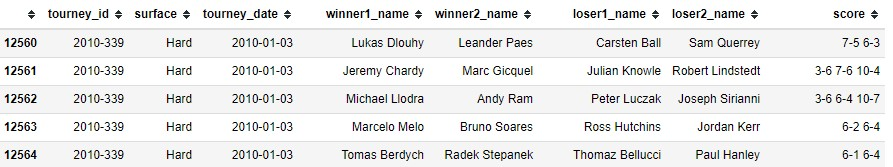
\includegraphics[width=400pt]{image/dataset.jpg}
\caption{ATP雙打-部分比賽資料}
\label{fig:double}
\end{figure}

男子職業雙打比賽可以分成四大網球公開事、ATP世界巡迴賽總決賽、ATP世界巡迴賽1000大師系列賽、ATP世界巡迴賽500系列賽事、ATP世界巡迴賽250系列賽等,而每一個系列賽或是公開賽會有對應的網球比賽制度,有些系列賽會採取小組循環賽,小組前幾名則晉級下一輪,例如:ATP世界巡迴賽總決賽,有些則是採取單敗淘汰賽制,比賽獲勝者則晉級下一輪,例如:四大網球公開賽,這些賽制皆有共通點,越靠近系列賽的尾部,代表參賽隊伍皆是贏得前面的比賽,也意味著強隊遇到強隊,彼此之間的實力差距應差異不大。
\section{分析結果}

我們首先討論在不同模型下,各別設置不同的參數來配適模型,並在不同的評估準則下,判斷不同的參數設定下,模型預測的表現能力。

\subsection{參數設定}

本篇研究結合了Ingram\cite{Ingram+2021}的GenElo surface model與 Weng \& Lin \cite{JMLR:v12:weng11a}的多組別多組員之實力更新方法,預測網球雙打比賽結果。兩者模型皆有一些超參數需要被設定,透過優化(optimize)的方式,找出較佳的超參數設定,讓模型在預測能力上有更好的表現。

在第3.3節中Bradley-Terry Model(Full-pair)模型需要設定
初始參數有每隊中參賽者實力$\mu_{ij}$、參賽者實力的變異數$\sigma^2_{ij}$、比賽中不可控制的變異數$\beta^2$、控制因子$\kappa$與$\gamma_q$,參考第2.1節中的參數設定,本研究將新進選手的實力$\mu_{ij}$初始值設為1500,比賽中不可控制的變異數設為9,控制因子$\kappa$設為0.0001,參考Weng \& Lin$\citep{JMLR:v12:weng11a}$的設定,將$\gamma_q$設置為$\dfrac{1}{2}$,參賽者實力的變異數$\sigma^2_{ij}$,則透過以下的方式進行優化。

本研究採用最小化交叉熵(cross-entropy)的方式進行優化,交叉熵為一種在分類問題中常見的損失函數,透過此優化方式,將訓練集的比賽資料進行訓練,找出適當的初始參賽者實力的變異數$\sigma^2_{ij}$,讓預測結果越能貼近比賽真實結果。每一場比賽中的交叉熵如下:
\begin{equation}
d_{iq}= -s_{iq}log(p_{iq})-(1-s_{iq})log(1-p_{iq})\label{cross}
\end{equation}
其中
\[
p_{iq} = \dfrac{e^{\mu_i/c_{iq}}}{e^{\mu_i/c_{iq}} +e^{\mu_q/c_{iq}}}
\]
\[
c_{iq} = (\sigma^2_i+\sigma^2_q + 2\beta^2)^{0.5}
\]
\[
\sigma^2_{i} = \Sigma_{j=1}^2\sigma^2_{ij}
\]
在(\ref{cross})式中$d_{iq}$代表比賽的交叉熵,$s_{iq}$代表第$i$隊遇上第$q$隊的比賽結果,$p_{iq}$代表第$i$隊隊伍擊敗第$q$隊隊伍的機率,所有的交叉熵則由每場比賽中的交叉熵進行加總而來,即為$\Sigma{d_{iq}}$,因為所有的交叉熵難以對$\sigma^2_{ij}$微分,故本研究採用由Nelder和Mead$\cite{nelder1965simplex}$所提出的Nelder-Mead方法,其能協助找尋極小值,並找尋到較佳的$\sigma^2_{ij}$,本次研究估計$\sigma^2_{ij}$時,其結果為3.55。

在第3.4節中Generalize Bradley-Terry Surface Model模型需要設定的初始參數有每隊中參賽者實力$\mu_{ijk}$、比賽中不可控制的變異數$\beta^2$、參賽選手在各場地發揮實力的變異數$\sigma^2_k$與在各場地間的相關係數$\rho_{12}$、$\rho_{23}$與$\rho_{13}$,此研究亦將每隊中參賽者實力$\mu_{ijk}$設置為1500,比賽中不可控制的變異數$\beta^2$設為9,參賽選手在各場地發揮實力的變異數$\sigma^2_k$與在各場地間的相關係數$\rho_{12}$、$\rho_{23}$與$\rho_{13}$,則透過優化的方式來取得。

本次優化方式亦採取最小化交叉熵,每一場比賽中的交叉熵$d_{iqk}$如下:
\begin{equation}
d_{iqk} = -s_{iqk}log(p_{iqk})-(1-s_{iqk})log(1-p_{iqk})
\label{entropy}
\end{equation}
其中
\[
p_{iqk} =  \dfrac{e^{\mu_{ik}/c_k}}{e^{\mu_{ik}/c_k}+e^{\mu_{qk}/c_k}}
\]
\[
c_{k} = (\sigma^2_k + \sigma^2_k + 2\beta^2)^{0.5}
\]
\[
\boldsymbol{\mu'_{\theta} = \mu_{\theta} - \textit{H}^{-1}(\mu_{\theta})j(\mu_{\theta})}
\]
在(\ref{entropy})式中,$s_{iqk}$表示第$i$隊與第$j$隊在場地$k$的比賽結果,$p_{iqk}$則代表代表第$i$隊隊伍在場地$k$擊敗第$q$隊隊伍的機率,將每一場比賽的交叉熵進行加總形成所有的交叉熵,即為$\Sigma{d_{iqk}}$,所有的交叉熵會隨著每一場參賽者實力的變動受到影響,參賽者實力的調整會受到先前比賽的結果而有所變動,而當該場地比完賽時,除了參賽者在該場地發揮的實力會做到調整以外,參賽者在其他場地發揮的實力亦會受到調整,因此所有的交叉熵難以對$\sigma^2_k$、$\rho_{12}$、$\rho_{23}$與$\rho_{13}$偏微分,故選擇用由Nelder \& Mead$\cite{nelder1965simplex}$所提出的Nelder-Mead方法,能找到($\sigma^2_1$,$\sigma^2_2$,$\sigma^2_3$,$\rho_{12}$,$\rho_{13}$,$\rho_{23}$)的組合,並使交叉熵達到最小。

\begin{table}[h!]
\caption{選手在不同場地上發揮實力的變異數與相關係數}
\centering
\begin{tabular}[center]{cccccc}
\hline
$\sigma^2_{clay}$ & $\sigma^2_{grass}$ & $\sigma^2_{hard}$ & $\rho_{clay-grass}$ & $\rho_{clay-hard}$&$\rho_{grass-hard}$\\
\hline
41.00 & 250.37 & 29.79 & 0.57&0.92&0.88\\
\hline
\end{tabular}
\label{table:surface}
\end{table}

表\ref{table:surface}為選手在不同場地上發揮實力的變異數與相關係數的組合,其為透過Nelder-Mead方法,將所有的交叉熵$\Sigma{d_{iqk}}$達最小的($\sigma^2_1$,$\sigma^2_2$,$\sigma^2_3$,$\rho_{12}$,$\rho_{13}$,$\rho_{23}$)組合,由表\ref{table:surface}可知,相關係數皆為正,代表當選手在比賽場地發揮的實力有正向的調整時,在其他場地發揮的實力也會有正向的調整,草地的變異數相較於其他場地的變異數還要大,這種情況也是合理的,草地的場地會因為天氣的狀況不同,影響球速也有所不同,此外,相較於其他場地,草地較容易出現一些不規則彈跳,會影響到比賽選手實力的發揮。
\subsection{評估準則}
為了能夠有效比較出不同模型的預測能力,我們這次採用統計學與機器學習上常用的指標,分別為準確度(Accuracy)與mean log-likelihood這兩種指標當作模型的評估準則,這次透過模型預測比賽結果與實際比賽結果比較,計算出此模型能成功預測比賽結果的比例,其代表模型的準確度,若準確度越高,代表模型有愈好的預測能力。我們採用mean log-likelihood考慮模型預測比賽結果的機率,若兩個參賽者實力懸殊,則應預測實力較強的選手有較高的勝率。

\subsection{模型預測結果}
\subsubsection{多組別多隊員之比賽}
在測試集中,將Bradley-Terry Model with full-pair預測比賽結果,並且評估每場比賽勝隊與敗隊的實力,接著將結果呈現於圖\ref{fig:b-t}。圖\ref{fig:b-t}的左半部為每一場比賽勝隊與敗隊的實力分布圖,其中橘點代表勝隊的實力大於敗隊的實力,亦即代表此模型預測成功的部份,反之,藍點代表勝隊的實力小於敗隊的實力,亦即代表此模型預測錯誤的部份,由此圖可知,由於大部分的點為橘色的,代表大致而言,模型預測結果是正確的。圖\ref{fig:b-t}的右半部為兩隊平均實力差距的直方圖,橘色與藍色分別代表勝隊的實力大於敗隊的實力與勝隊的實力小於敗隊的實力,由圖可知,隨著兩隊平均的實力差距越大,可看出橘色的部分佔的比例增加,代表模型預測比賽結果更加準確,換而言之,當兩隊的平均實力差異不大時,比較難預測比賽結果。

\begin{figure}[h!]
\centering
\subfigure{
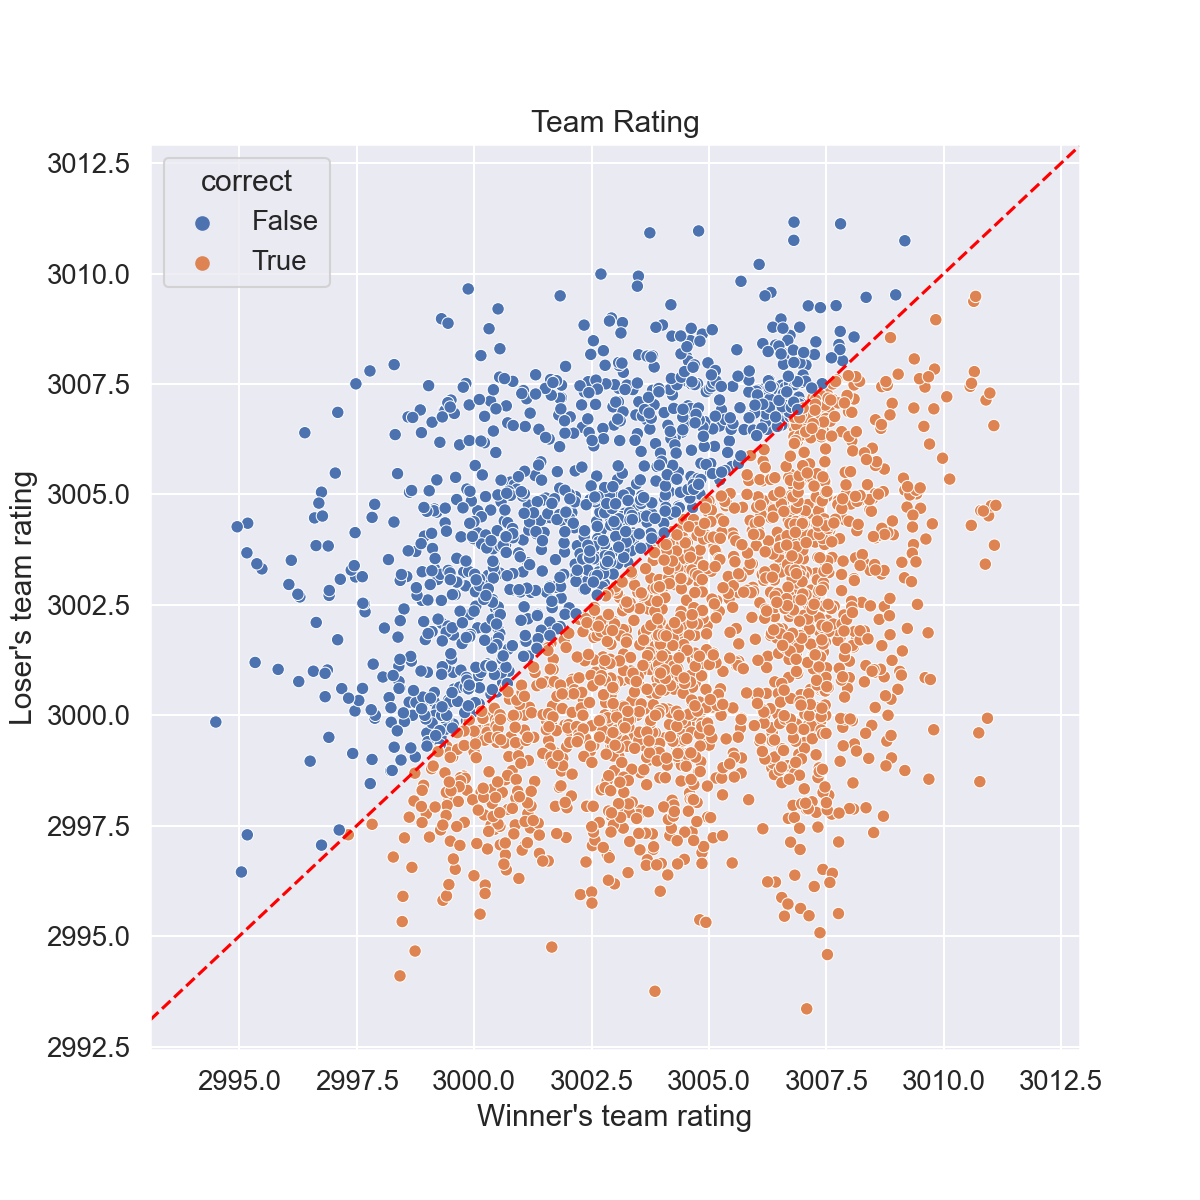
\includegraphics[width=110pt]{image/b-t_rating.png}
}
\subfigure{
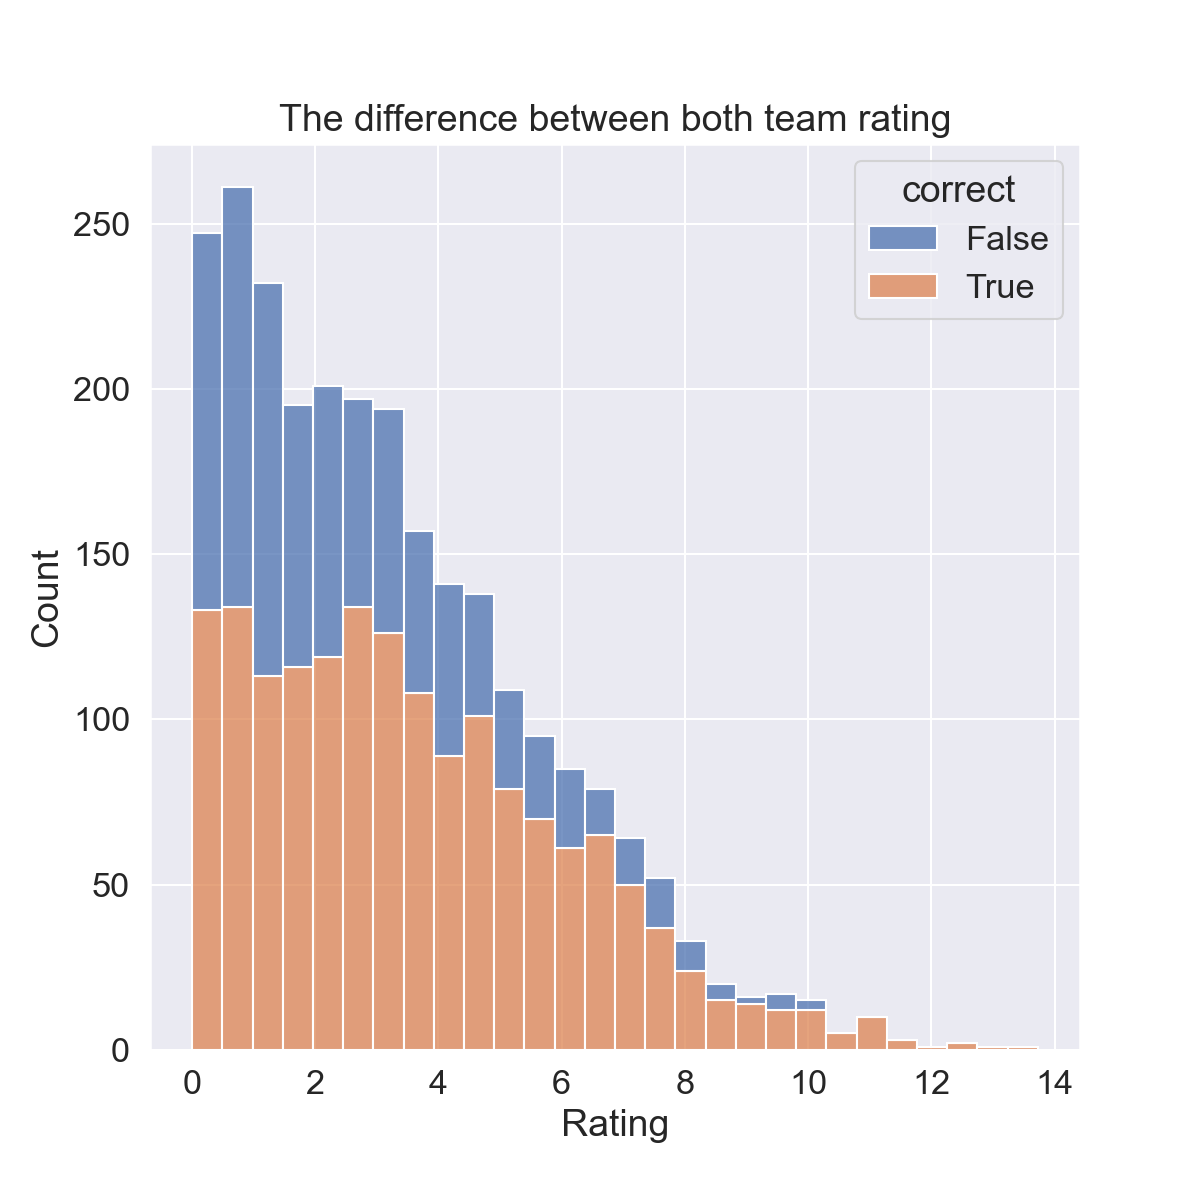
\includegraphics[width=110pt]{image/b-t_rating_diff.png}
}
\caption{在測試集上,用Bradley-Terry Model with full-pair評估每場比賽中勝隊與敗隊的實力。}
\label{fig:b-t}
\end{figure}
\subsubsection{結合場地於雙打比賽}
在測試集中,利用本論文所提出的模型預測比賽結果,並且評估每一場比賽的敗隊與勝隊的實力,並且將結果呈現於圖\ref{fig:surface_hard}。圖\ref{fig:surface_hard}由上至下分別是在比賽場地為紅土、草地、硬地下,每場比賽勝隊與敗隊實力分布情況,由左至右分別為在該場地下,勝隊與敗隊實力分布和兩隊實力之間的差距,橘色代表該比賽中預測勝隊的實力大於預測敗隊的實力,藍色則代表該比賽中預測勝隊的實力小於預測敗隊的實力。由圖\ref{fig:surface_hard}的上半部可知,不論比賽場地為何種,橘色的點皆比藍色的點還要多,大致而言,模型預測比賽結果是正確的。由圖\ref{fig:surface_hard}的右半部可知,不論比賽場地為何種,皆可發現隨著兩隊的實力差距越大,可以看出橘色的部分所佔的比例增加,代表模型愈能預測比賽結果,此外,我們發現當比賽場地為草地時,相較於其他場地,兩隊實力的差距分布較廣,其原因可從表\ref{table:surface}觀察出$\sigma^2_{grass}$明顯比$\sigma^2_{clay},\sigma^2_{hard}$大上不少。

\begin{figure}[h!]
\subfigure{
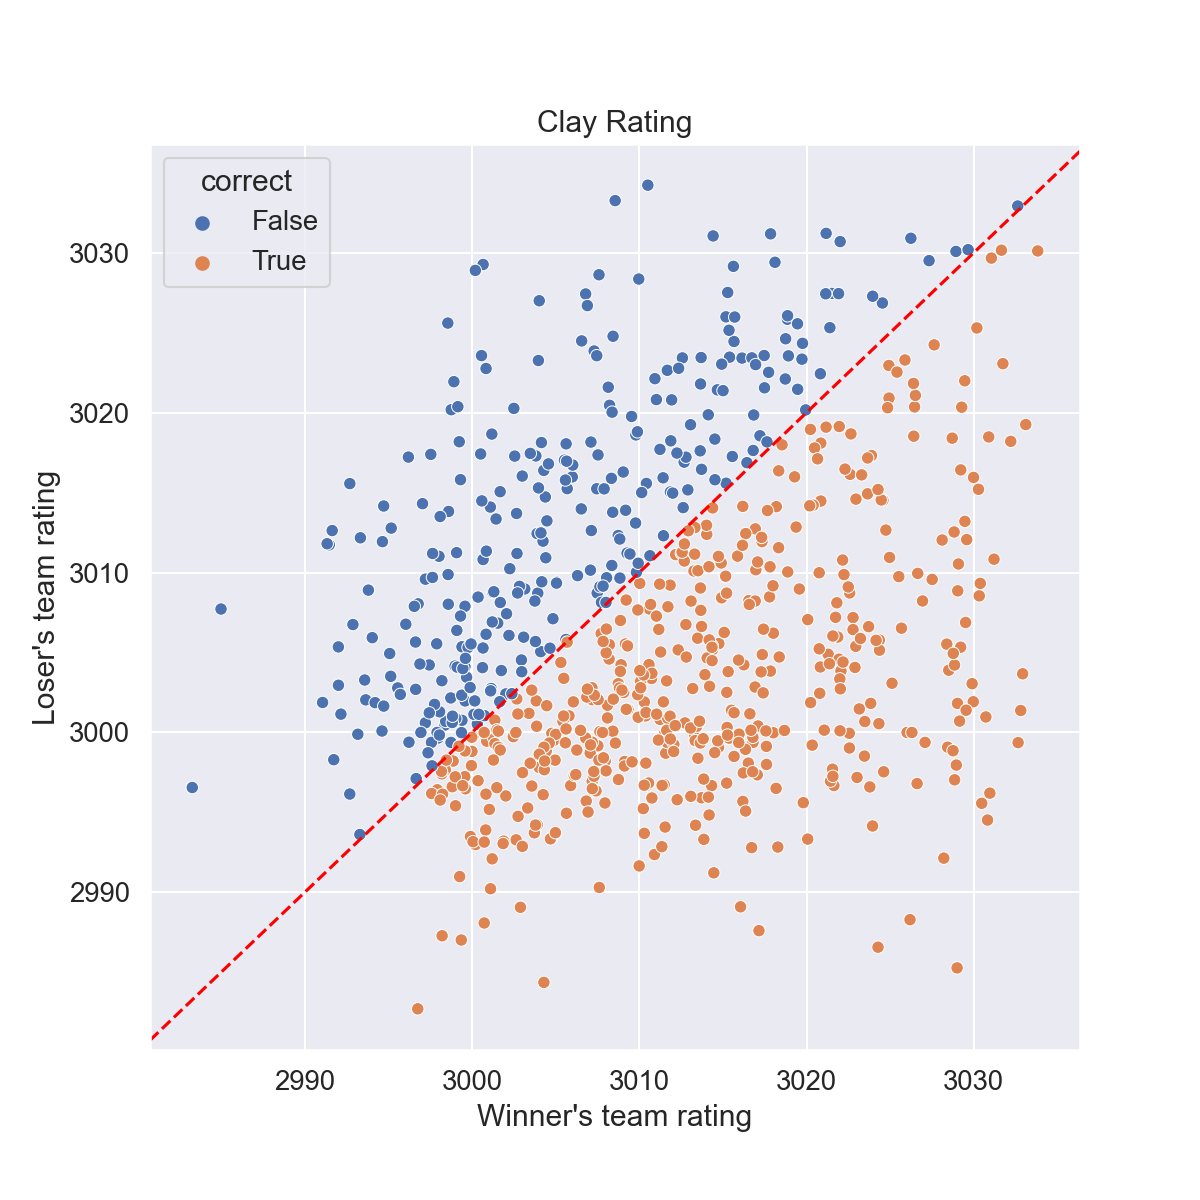
\includegraphics[width=175pt]{image/clay_rating.png}
}
\subfigure{
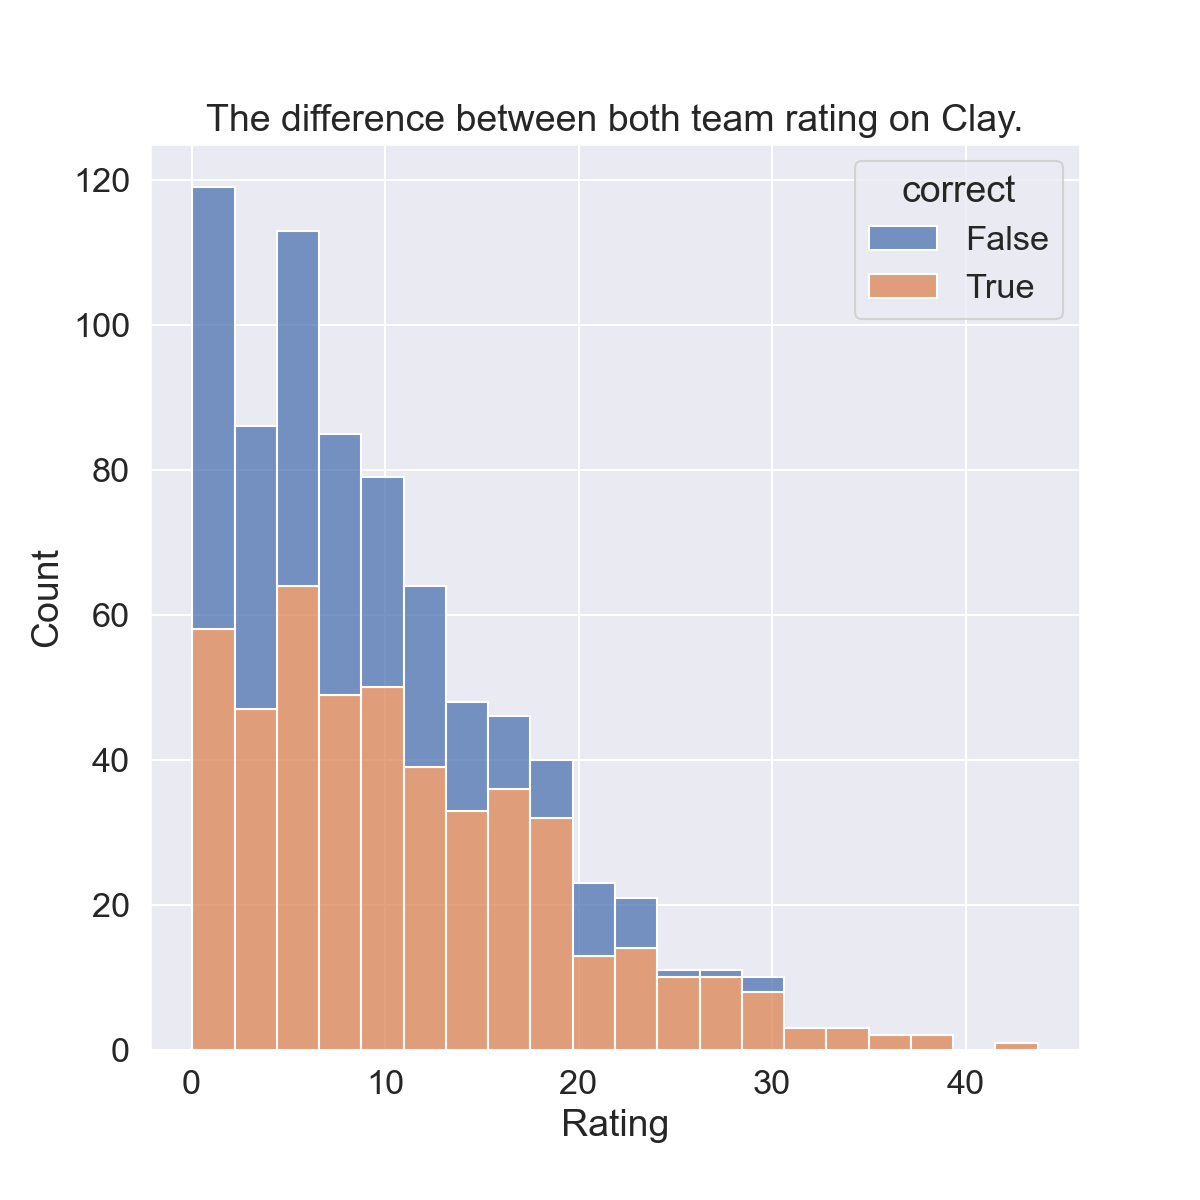
\includegraphics[width=175pt]{image/clay_rating_diff.png}
}
\label{fig:surface_clay}
\end{figure}
\begin{figure}[h!]
\subfigure{
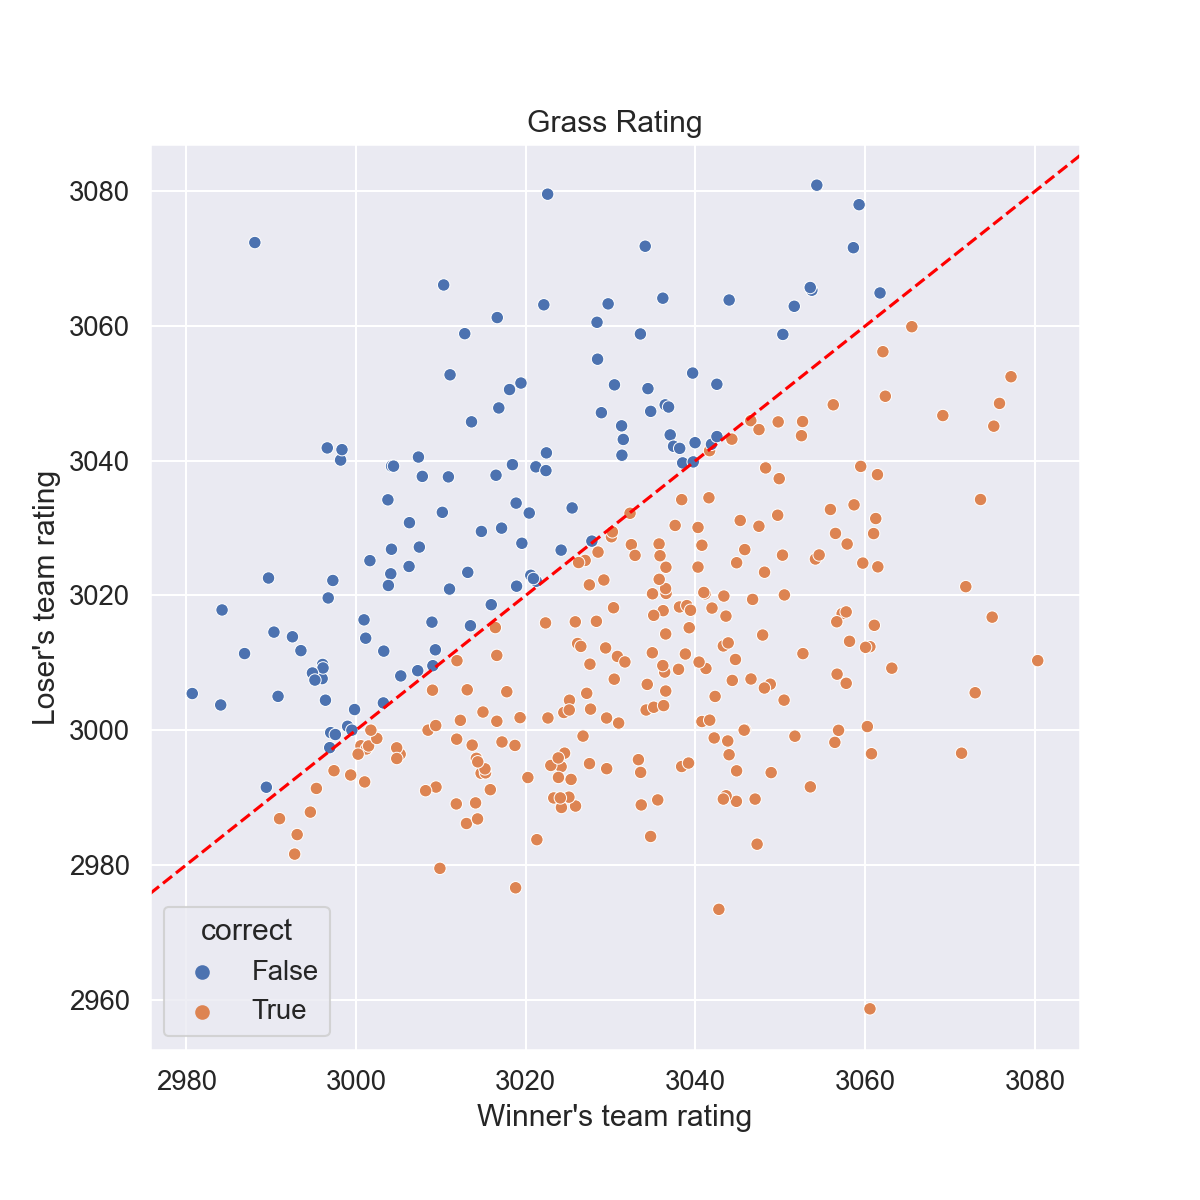
\includegraphics[width=175pt]{image/grass_rating.png}
}
\subfigure{
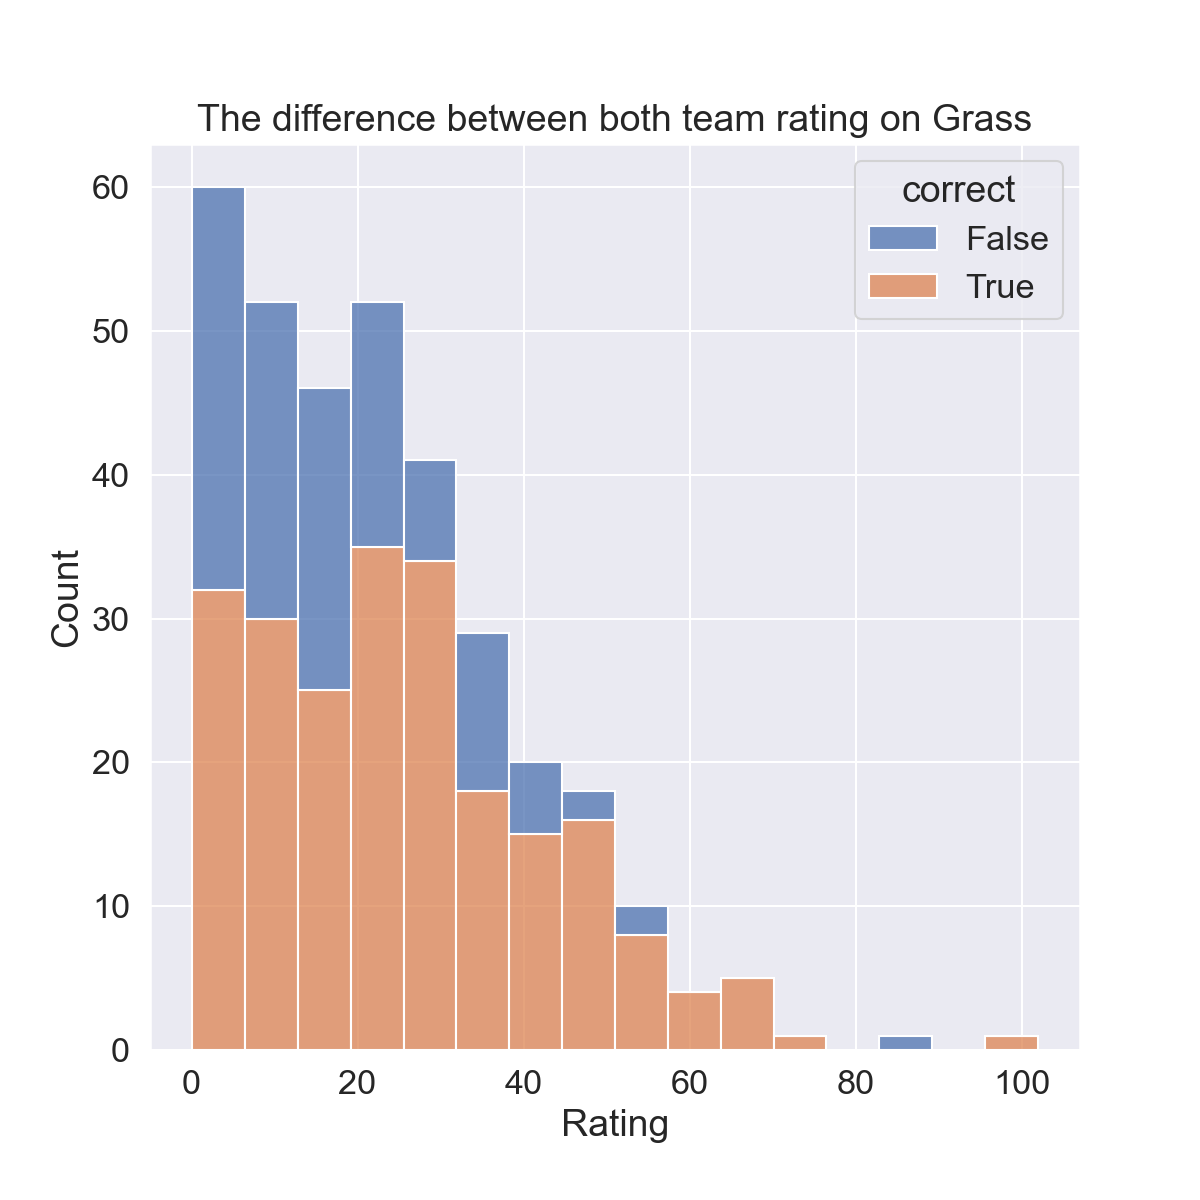
\includegraphics[width=175pt]{image/grass_rating_diff.png}
}
\label{fig:surface_grass}
\end{figure}
\begin{figure}[h!]
\subfigure{
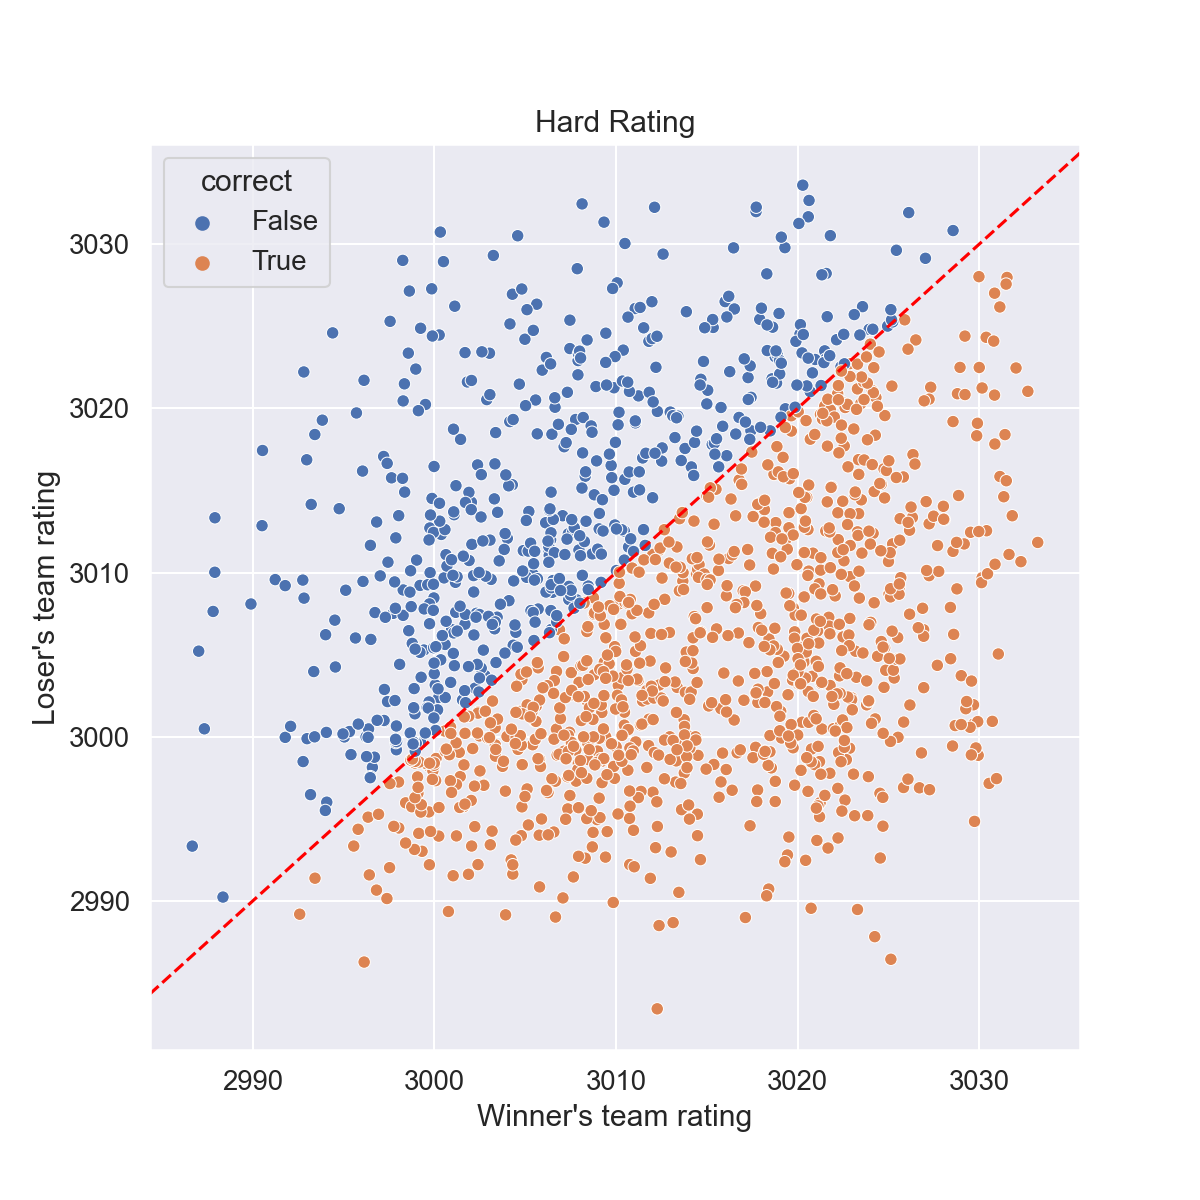
\includegraphics[width=175pt]{image/hard_rating.png}
}
\subfigure{
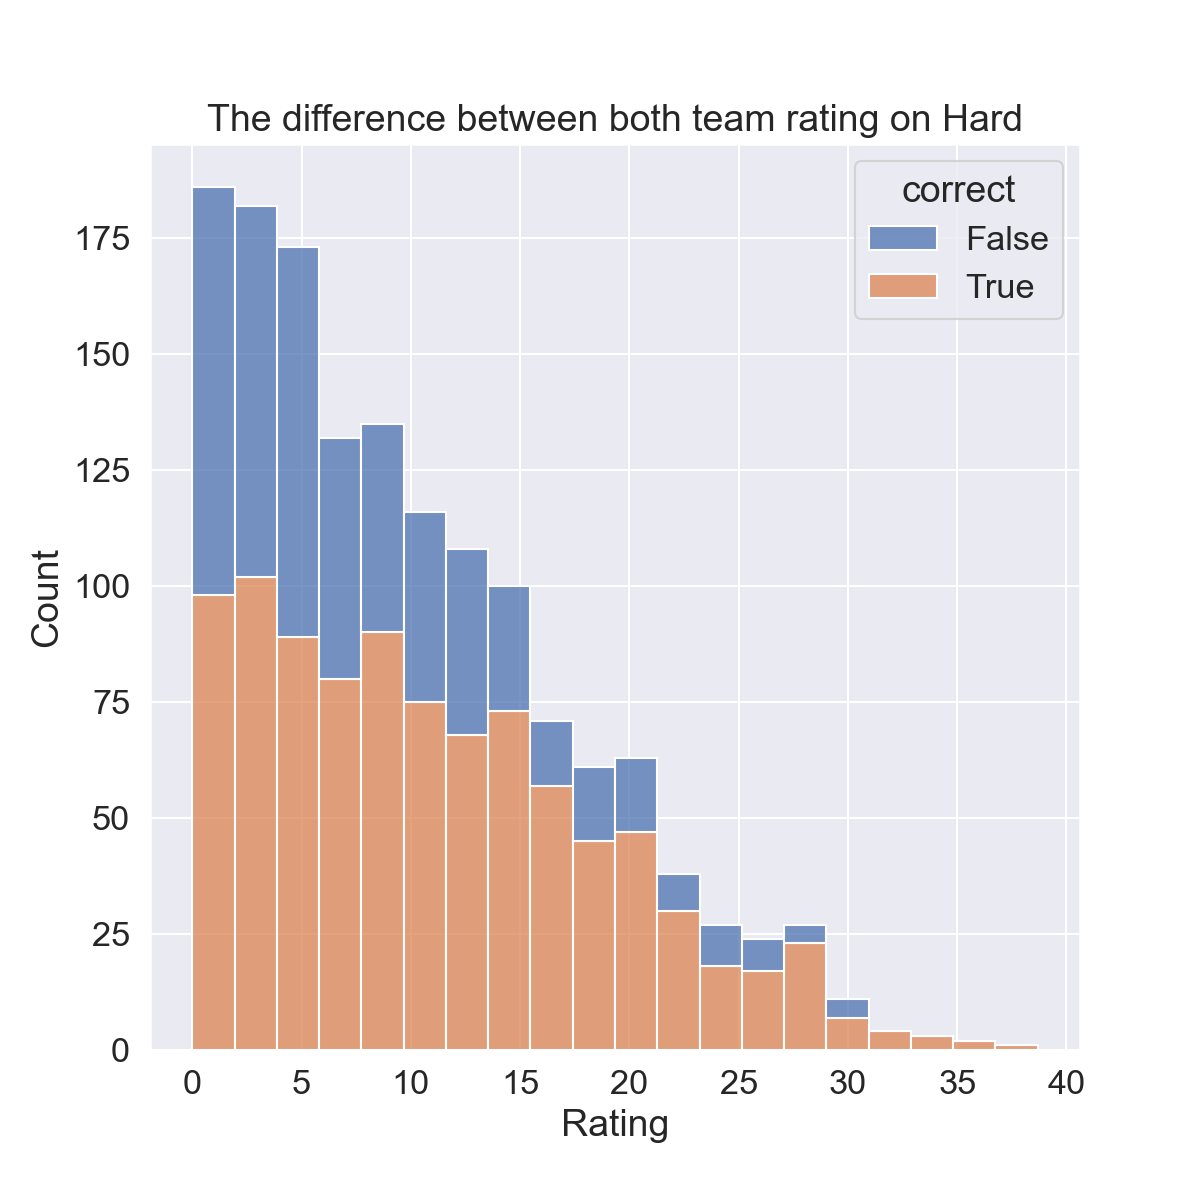
\includegraphics[width=175pt]{image/hard_rating_diff.png}
}
\caption{在測試集上,用本論文提出的模型分別在紅土、草地與硬地的比賽場地中,評估每場比賽中勝隊與敗隊的實力。}
\label{fig:surface_hard}
\end{figure}

\clearpage
\subsubsection{整體}
表\ref{model:predict}為模型在訓練集訓練完參數後,在測試集中,評估各模型的準確度與mean log-likelihood,在準確度方面而言,Bradley-Terry Model (Full-pair)模型的準確度達$0.6359$,略為高於Generalize Bradley-Terry Surface Model的準確度$0.6328$,在mean log-likelihood方面而言,Bradley-Terry Model (Full-pair)的mean log-likelihood達-0.6393也略大於Generalize Bradley-Terry Surface Model的mean log-likelihood達-0.6692,整體而言,Bradley-Terry Model (Full-pair)皆略勝於Generalize Bradley-Terry Surface Model,其原因歸自於在Bradley-Terry Model (Full-pair)有考慮到不同參賽選手間發揮實力的變異性,而Generalize Bradley-Terry Surface Model假設每位選手間發揮實力的變異性皆相同,故Bradley-Terry Model (Full-pair)在測試集上有較佳的預測能力。
\begin{table}[!h]
\caption{在測試集中,評估模型預測的能力}
\centering
\begin{tabular}[center]{ccc}
\hline
Model & Accuracy & Mean log-likelihood\\
\hline
Bradley-Terry Model (Full-pair) & 0.6359 & -0.6393\\
Generalize Bradley-Terry Surface Model & 0.6328 & -0.6692 \\
\hline
\end{tabular}
\label{model:predict}
\end{table}

\section{結論與建議}
本研究以男子職業網球比賽為例,藉由評分模型探討網球雙打選手的技能,並考慮比賽場地的因素,評估每隊在各種場地下所發揮的實力,從模型訓練的過程中,藉由訓練資料集估計超參數,接續在固定超參數的情況下,從測試集中預測比賽兩隊各別獲勝的機率,藉此預測哪隊為獲勝的隊伍。

在過去研究配對比較模型中,Weng \& Lin曾提出Bradley-Terry Model with full-pair 與partial pair\cite{JMLR:v12:weng11a}評分模型,將該模型運用於ATP雙打資料集上,與本研究進行比較,預測準確度從0.6359略下降至0.6328,Mean log-likelihood亦從-0.6393下降至-0.6692,本研究所採用的模型表現並未比較好,但本研究所採用的模型可透過共變異數矩陣$\boldsymbol{\Lambda}$可得知不同場地間會有關聯性,在關聯程度上紅土與草地是相對低的,也驗證了紅土的特性在於球速慢,草地的特性在於球速快,兩者場地的特性極為不同。



雖然本研究是運用在網球的資料上,但一般而言,本研究可以同應運用在其他運動比賽上,比方在沙灘排球方面,Glickman \& Hennessy \& Bent\cite{glickman2018comparison}曾利用Elo、Glicko等評分系統評估女子沙灘排球的排名,同樣的道理,本研究亦可以套用在女子沙灘排球上,並且評估每隊的實力。

\bibliography{ref.bib}%參考文獻檔名

\end{document}
